\section{Methods}

\subsection{System Architecture}

The Agentic USMLE Study Planning System employs a stateful graph architecture implemented using LangGraph \cite{langgraph2024}. The system decomposes the tutoring task into four specialized agents that communicate through a typed state object, enabling modularity, testability, and clinical oversight.

\subsubsection{Graph Structure}

The agentic graph follows a directed acyclic structure with conditional branching (Figure \ref{fig:graph_architecture}):

\begin{verbatim}
START --> Diagnostician --> KnowledgeManager --> ResourceOptimizer --> Scheduler
                                                                               |
                                                                               v
                                        +--------------------------------------+------+
                                        |                                            |
                                        v                                            v
                                HumanReview (conditional)                       Finalize
                                        |                                            |
                                        +--------------------------------------------+
\end{verbatim}

\begin{figure}[H]
\centering
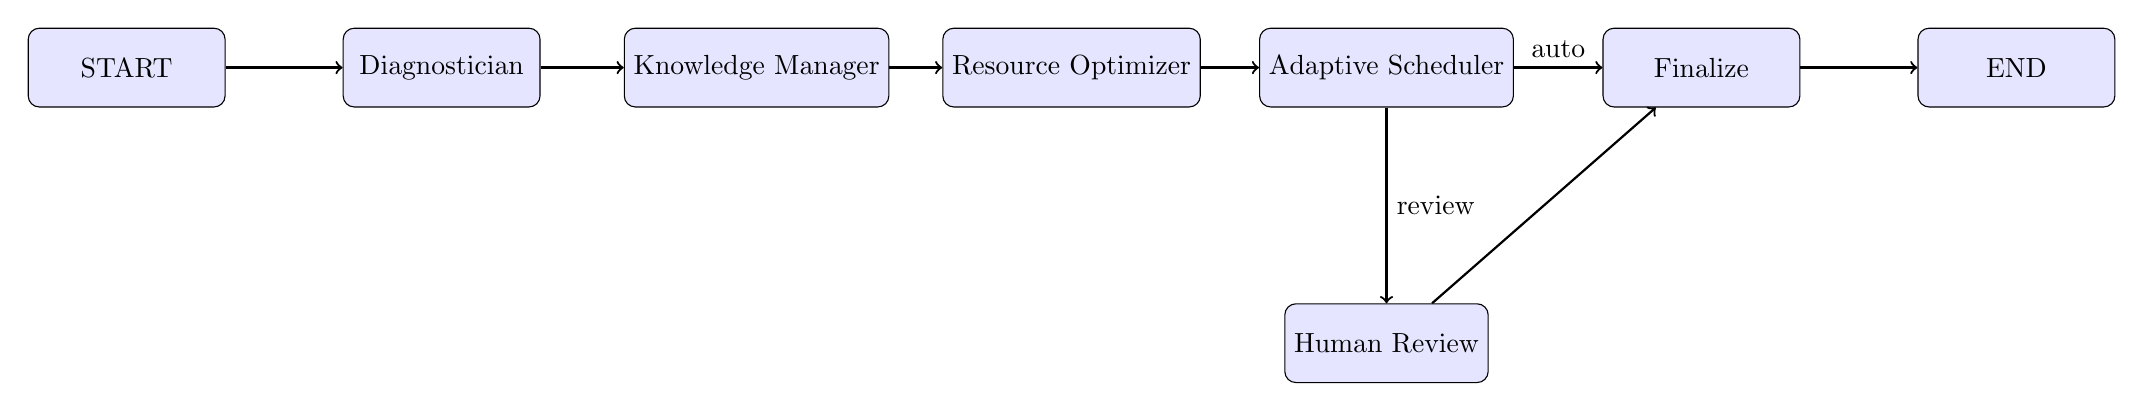
\begin{tikzpicture}[
    node distance=2cm,
    box/.style={rectangle, draw, fill=blue!10, rounded corners, minimum width=2.5cm, minimum height=1cm},
    arrow/.style={->, thick}
]
\node[box] (start) {START};
\node[box, right of=start, xshift=2cm] (diag) {Diagnostician};
\node[box, right of=diag, xshift=2cm] (know) {Knowledge Manager};
\node[box, right of=know, xshift=2cm] (rag) {Resource Optimizer};
\node[box, right of=rag, xshift=2cm] (sched) {Adaptive Scheduler};
\node[box, below of=sched, yshift=-1.5cm] (review) {Human Review};
\node[box, right of=sched, xshift=2cm] (final) {Finalize};
\node[box, right of=final, xshift=2cm] (end) {END};

\draw[arrow] (start) -- (diag);
\draw[arrow] (diag) -- (know);
\draw[arrow] (know) -- (rag);
\draw[arrow] (rag) -- (sched);
\draw[arrow] (sched) -- node[above] {auto} (final);
\draw[arrow] (sched) -- node[right] {review} (review);
\draw[arrow] (review) -- (final);
\draw[arrow] (final) -- (end);
\end{tikzpicture}
\caption{Multimodal Agentic Graph Architecture. The Resource Optimizer (Agent 2) performs multimodal RAG retrieval before the Scheduler generates plans with specific resource recommendations.}
\label{fig:graph_architecture}
\end{figure}

\subsubsection{Agent A: Diagnostician}

The Diagnostician agent parses raw NBME and UWorld performance reports using Groq's Llama-3.1-70B model. The agent employs structured prompting with few-shot examples to extract:

\begin{itemize}
    \item Overall performance metrics (NBME 3-digit score, UWorld percentile)
    \item Weak knowledge areas (proficiency $< 60\%$)
    \item Strong knowledge areas (proficiency $> 75\%$)
    \item Specific knowledge gaps with severity scores (0.0 to 1.0)
    \item Recommended focus areas ordered by priority
\end{itemize}

The system prompt encodes domain expertise about USMLE subject weights and IMG-specific challenges. Temperature is set to 0.2 for deterministic, consistent output. The agent returns JSON conforming to a typed schema (Pydantic model), ensuring downstream agents receive structured data.

\subsubsection{Agent B: Knowledge Manager}

The Knowledge Manager maintains a persistent ``knowledge vector'' for each student in Supabase, a PostgreSQL-based database with pgvector extension for embedding support. This agent serves as the system's memory, reading historical performance data and updating proficiency scores.

Proficiency updates use an exponential moving average model:

\begin{equation}
P_{t+1} = (1 - \alpha) \cdot P_t + \alpha \cdot (A_{session} \times 100)
\end{equation}

where $P_t$ is current proficiency, $\alpha = 0.15$ is the learning rate, and $A_{session}$ is the session accuracy. The agent also calculates a predicted USMLE score using weighted area proficiencies mapped to the 3-digit scale.

\subsubsection{Agent C: Multimodal Resource Optimizer (RAG)}

The Resource Optimizer is the novel contribution of this work—a multimodal RAG engine that retrieves and recommends USMLE study resources across five modalities:

\paragraph{Supported Modalities.}
\begin{enumerate}
    \item \textbf{Text}: First Aid chapters, UWorld explanations, clinical notes, study guides
    \item \textbf{Images}: Pathology slides (H\&E stained sections), ECG strips (AFib, VTach, heart blocks), radiographs (CXR findings), diagrams (metabolic pathway maps), tables (drug classifications)
    \item \textbf{PDFs}: NBME score reports, USMLE content outlines, IMG preparation guides, official practice exams
    \item \textbf{Video}: Pathoma lectures (Dr. Sattar), Boards \& Beyond (Dr. Ryan), SketchyMedical visual mnemonics—with timestamp-level retrieval for specific segments
    \item \textbf{Audio}: USMLE podcast episodes, lecture recordings, transcript summaries for passive learning
\end{enumerate}

\paragraph{Resource Database.}
The system maintains a curated database of 45+ USMLE resources, each annotated with:
\begin{itemize}
    \item Modality-specific metadata (page ranges for text, timestamps for video, image descriptions for pathology/ECG)
    \item Clinical relevance tier (essential, high-yield, supplementary, reference)
    \item Topic and area tags for retrieval matching
    \item IMG-specific flags for resources addressing IMG knowledge gaps (US healthcare system, reference lab values)
    \item Engagement metrics (student ratings, usage counts) for social proof scoring
\end{itemize}

\paragraph{Retrieval Algorithm.}
The RAG engine uses a multi-stage retrieval process:

\begin{enumerate}
    \item \textbf{Stage 1 - Topic Scoring:} Each resource is scored based on topic match to the query area and specific topic:
    \begin{equation}
    S_{topic} = w_1 \cdot \mathbb{I}_{area} + w_2 \cdot \text{sim}_{desc} + w_3 \cdot \text{sim}_{topic} + w_4 \cdot \sum \text{sim}_{tags}
    \end{equation}
    where $\mathbb{I}_{area}$ is the exact area match indicator and $\text{sim}$ functions measure text overlap.
    
    \item \textbf{Stage 2 - Modality Balancing:} The system ensures at least one resource from each relevant modality (text, image, video, qbank) is included, providing a multimodal learning experience.
    
    \item \textbf{Stage 3 - Constraint Filtering:} Resources are filtered by available study time, learning style preference (visual/auditory/reading), and IMG status.
    
    \item \textbf{Stage 4 - Ranking:} Final resources are ranked by combined relevance score including tier priority, student ratings, and usage popularity.
\end{enumerate}

For production deployment, Stage 1 would use vector similarity search with OpenAI ada-002 embeddings (1536-dim) for text and CLIP ViT-L/14 embeddings (768-dim) for images, stored in Supabase pgvector with IVFFlat indexes for efficient nearest-neighbor retrieval.

\paragraph{IMG-Specific Optimization.}
The Resource Optimizer boosts IMG-specific resources when the student is identified as an IMG. These include:
\begin{itemize}
    \item US healthcare system guides (insurance types, referral systems)
    \item US laboratory reference value tables (which may differ from international ranges)
    \item NBME score report interpretation guides
    \item ECFMG registration and requirements documentation
\end{itemize}

\subsubsection{Agent D: Adaptive Scheduler}

The Adaptive Scheduler generates 7-day (configurable) study blocks encoding three evidence-based learning strategies, enhanced with multimodal resource recommendations from Agent C:

\paragraph{Interleaved Practice.}
Rather than blocking single topics per day, the scheduler alternates between different subjects within each day, implementing Rohrer and Taylor's findings \cite{rohre2007interleaving}. Our implementation interleaves weak and strong areas, and the Resource Optimizer ensures each block includes resources from multiple modalities.

\paragraph{Spaced Repetition.}
Every third day is designated as a ``review day,'' scheduling comprehensive review of previously studied material at expanding intervals (1, 3, 7, 14 days) following Cepeda et al.'s spacing effect research \cite{cepeda2008spacing}.

\paragraph{Active Recall.}
Each study block includes 20-40 practice questions, implementing Karpicke and Roediger's testing effect \cite{karpicke2008retrieval}.

The scheduler can operate in LLM mode (Groq/Llama-3.1 for natural language rationale) or heuristic mode (rule-based fallback for reliability).

\subsection{Database Schema}

The system uses Supabase (PostgreSQL with pgvector) for persistent storage with the following core tables:

\begin{itemize}
    \item \texttt{students}: Demographic and baseline data including learning style
    \item \texttt{knowledge\_areas}: USMLE subject taxonomy with subtopics
    \item \texttt{student\_knowledge}: Knowledge vectors with proficiency scores and text embeddings (1536-dim)
    \item \texttt{multimodal\_resources}: Resource catalog with text embeddings (1536-dim), image embeddings (768-dim), modality-specific metadata
    \item \texttt{student\_resource\_interactions}: Tracking which resources students actually used and their ratings
    \item \texttt{student\_uploads}: Student-uploaded documents (PDF score reports, images) with OCR-extracted text and embeddings
    \item \texttt{performance\_logs}: Session-level performance data
    \item \texttt{study\_plans}: Generated plans with JSON structure and multimodal flags
    \item \texttt{study\_blocks}: Individual daily blocks with resource modality arrays
    \item \texttt{agent\_executions}: Execution logs for debugging and research
\end{itemize}

Vector indexes use IVFFlat for approximate nearest neighbor search:
\begin{verbatim}
CREATE INDEX idx_resources_text_embedding 
    ON multimodal_resources USING ivfflat (text_embedding vector_cosine_ops);
CREATE INDEX idx_resources_image_embedding 
    ON multimodal_resources USING ivfflat (image_embedding vector_cosine_ops);
\end{verbatim}

Row Level Security (RLS) policies ensure students can only access their own data, while the multimodal resource catalog is publicly readable.

\subsection{Human-in-the-Loop Review}

The graph includes a conditional edge that routes to a HumanReview node when predicted score $< 180$, more than 3 weak areas are identified, or explicitly requested. This ensures clinical oversight for high-stakes decisions.

\subsection{Evaluation Methodology}

We evaluate the system through technical metrics (execution time, success rate), clinical plan quality (expert rubric scoring), and a pilot user study with 10-20 IMG students collecting pre/post NBME scores and qualitative feedback.

The multimodal RAG system is specifically evaluated on:
\begin{enumerate}
    \item \textbf{Modal coverage:} Does the plan include resources from at least 3 modalities?
    \item \textbf{Resource appropriateness:} Are recommended resources at the correct difficulty level?
    \item \textbf{IMG optimization:} Are IMG-specific resources included when relevant?
    \item \textbf{Time feasibility:} Do multimodal resource recommendations fit within allocated study time?
\end{enumerate}
